\section{Probabilistische Turingmaschinen}

\subsection{Definition}
Wir nutzen das Modell der Mehrband-Turingmaschine um abstrakt die Fähigkeit einer Turing-Maschine zu zeigen, eine zufällige Auswahl zu treffen, entsprechend einem Programm, das einen Zufallszahlengenerator einmal oder mehrfach aufruft.
Auf dem ersten Band steht wie bei einer Mehrband-Turingmaschine üblich die Eingabe.
Das zweite Band, das sogenannte \emph{Zufallsband}, ist vollständig mit den Symbolen $1$ und $0$, die zufällig und unabhängig voneinander mit der Wahrscheinlichkeit $P(x) = \frac{1}{2}, x \in \{0, 1\}$.
Die übrigen Bänder sind initial leer und können nach Bedarf als \emph{Hilfsbänder} genutzt werden.

\begin{figure}[h]
	\centering
	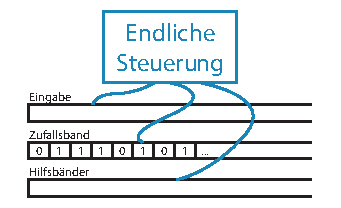
\includegraphics[width=.8\textwidth]{Graphics/Probabilistic_TM}	
\end{figure}

Wir nennen dieses Modell einer Turingmaschine \emph{zufallsabhängige Turingmaschine} oder \emph{probabilistische Turingmaschine}.


\subsection{Initialisierung des Zufallsbandes}
\paragraph{Beobachtung:}
Da die komplette Initialisierung des unendlichen Zufallsbandes mit den Symbolen $1$ und $0$ ist nicht realistisch, da diese nie terminiert.

\paragraph{Lösung:}
Das Zufallsband ist initial ebenfalls leer, enthält also nur \emph{Blanks}. 
Liest der Lese-Schreibkopf auf dem Zufallsband nun ein \emph{Blank}, so wird intern mittels eines Zufallsgenerators eine $1$ oder eine $0$ erzeugt und auf das Zufallsband geschrieben.
Das generierte Symbol wird anschließend nicht wieder verändert.
Auf diese Weise scheint das Zufallsband vollständig initialisiert.

\subsection{Beispiel: Probabilistischer Quicksort}


\subsection{Sprache}